\section{Background}\label{s:background}
We study parameter tuning for systems that address \emph{cell inconsistencies}, where record values are missing, incorrect, contain inconsistent references to the same entities, or contain artifacts from the extraction process. 

\subsection{Motivation}
Our goal is to develop techniques to automatically generate and tune data cleaning pipelines based on user-specified quality characteristics.  Thus, the user can primarily focus on composing and expressing data quality issues, and allow the system to explore the space of physical cleaning plans.  We would like the search procedure to be \textbf{progressive}, in the sense that it quickly generates acceptable cleaning plans, and refines those plans over time.  Thus, the user can immediately assess her hypothesis, or test multiple hypotheses in parallel.


\begin{figure}[t]
  \centering
 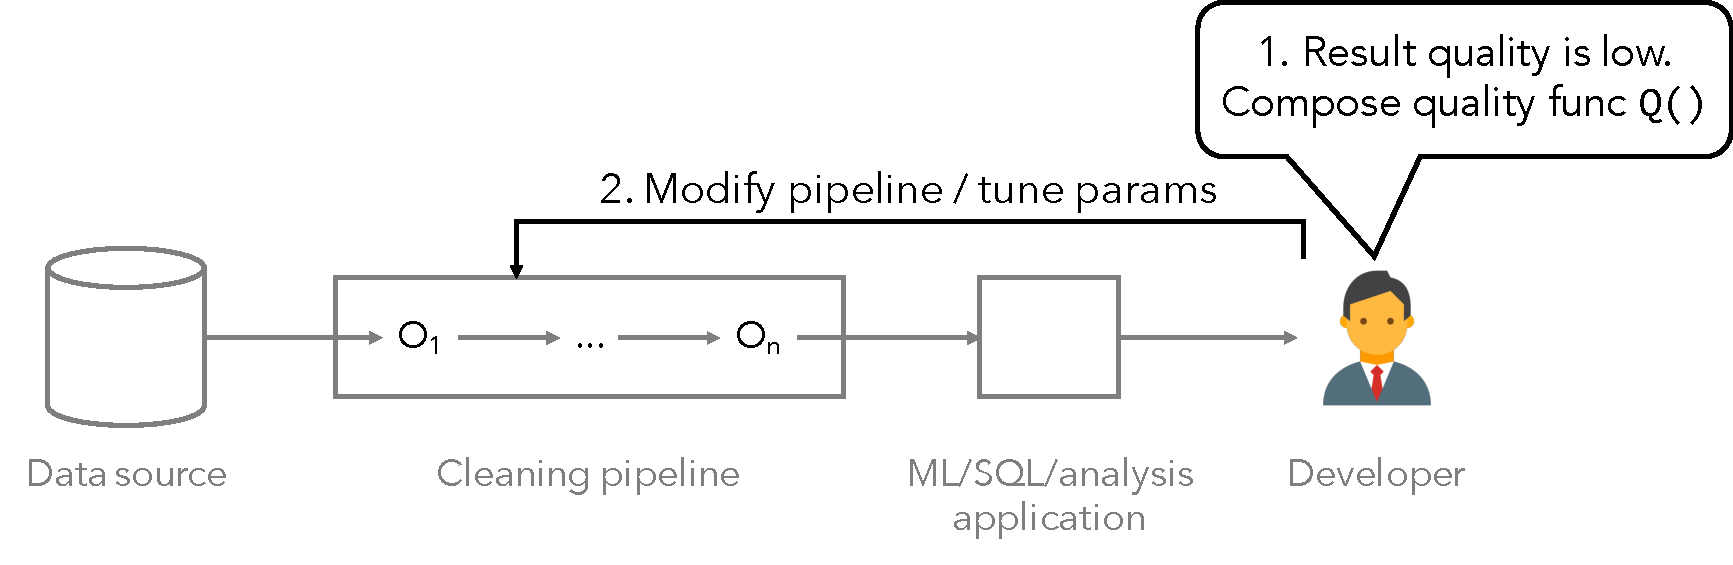
\includegraphics[width=\columnwidth]{figures/user-pipeline}
 \caption{\small Typical data cleaning pipeline.  The user finds that analysis results (of SQL query, ML model, web application, etc) are suspicious and iteratively (1) composes a quality function to characterize the suspicious quality issues, and (2) modifies the data cleaning pipeline to address the errors.  \sys improves this human-in-the-loop process by providing an expressive, composable quality function, and automatically searching for cleaning pipelines.  \label{fig:user-pipeline}}
\end{figure}

This iterative pattern makes data cleaning a human-in-the-loop problem, where the developer explores a large space of data quality issues {\it and} data cleaning programs (Figure \ref{fig:user-pipeline}).  However, the data cleaning systems ecosystem is diffuse, with separate systems for constraint resolution ~\cite{rekatsinas2017holoclean}, cleaning in machine learning pipelines~\cite{DBLP:journals/pvldb/KrishnanWWFG16}, entity resolution~\cite{mudgal2018deep, doan2018toward}, and crowdsourcing~\cite{DBLP:journals/pvldb/HaasKWF015}.
Each of these systems has its own idiosyncrasies and parameters, and tuning even one of these systems can be a daunting challenge.
Real-world datasets have mixes of errors~\cite{krishnan2016hilda} and often require multiple systems to clean~\cite{DBLP:conf/sigmod/ChuIKW16}.
Although these systems make it easier to construct and execute a pipeline, the space of possible operator pipelines and parameterizations of each operator is exponential in the number of operators, parameters, and pipeline depth, and is infeasible for developers to manually search.

\subsection{Challenges}
We could start by considering the recent work in \emph{hyperparameter tuning} for machine learning, which identifies the optimal assignment of hyperparameters to maximize an objective function (e.g., training accuracy for ML models).
Several systems have been built to run hyperpameter and neural network model search at scale~\cite{li2017hyperband, sparks2017keystoneml, baylor2017tfx, golovin2017google, liaw2018tune}.
For single threaded search, the state-of-the-art remains to be Bayesian optimization, e.g., Python Hyperopt~\cite{bergstra2013hyperopt}.
Since Bayesian optimization is inherently sequential, for parallel and distributed settings, the community is increasingly studying randomized and grid search schemes~\cite{li2017hyperband, liaw2018tune, golovin2017google}.
For a pipeline of up to $k$ cleaning components, we can create a parameter that represents the operator type in each of the pipeline slots, along with additional operators to tune each operator in each pipeline slot.  A hyperparameter tuning algorithm will then select and assign parameter values to a sequence of operators.
Although this approach is possible, it ignores important aspects of data cleaning problems that can enable more efficient and flexible approaches.  

\vspace{0.5em}
\noindent \textbf{Quality Function Structure. } Hyperparameter tuning algorithms are also called ``black-box'' optimization algorithms because they only assume oracular access to the optimization objective (i.e., evaluate the quality of a given plan). In contrast, the objectives in data cleaning have far more structure. 
If the objective is to minimize functional dependency violations, it would be wasteful to recompute all violations after every repair. One could incrementally evaluate update the objective from the set of modified keys.
This is also true in time-series data cleaning problem where quality measures are tied to certain windows of data--there is no point re-evaluating the whole objective if only a small window is affected.
In other words, data quality measures commonly support efficient incremental evaluation, and satisfy properties that enable data partitioning.  
Neglecting this structure leads to a large amount of duplicated effort for every parameter setting evaluated.

\begin{figure}[t]
\centering
 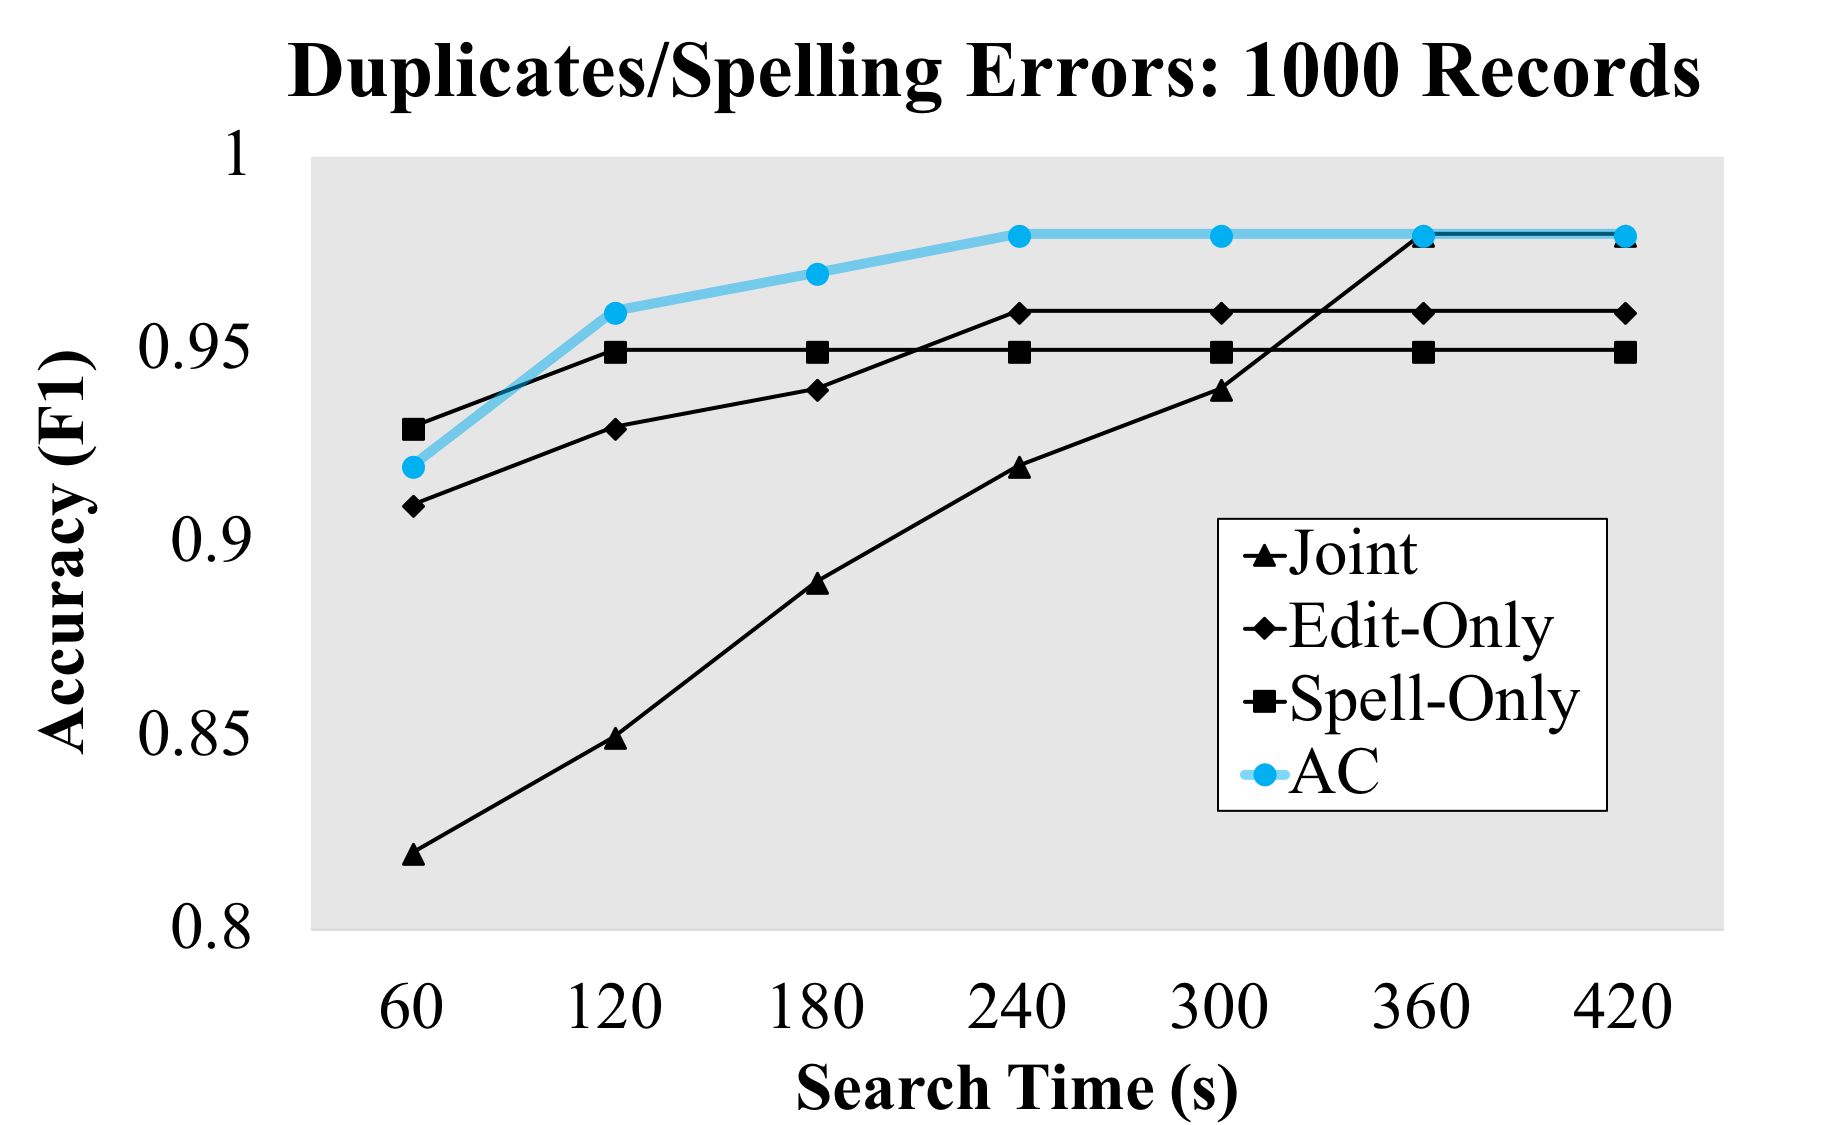
\includegraphics[width=0.9\columnwidth]{figures/teaser-experiment.png}
 \caption{\small 10\% of a dataset of dictionary words are duplicated with randomly generated spelling errors. The dataset is to be cleaned with a similarity matcher and a spell checker. Holistically, tuning the parameters of both with \textsf{python hyperopt} (BB-Full) is inefficient due to interactions between the two data cleaning options. It takes over 3x the amount of search time for the joint optimization to exceed the best tuned single cleaning method (BB-Edit and BB-SpellCheck) \label{fig:teaser}}
\end{figure}


\vspace{0.5em}
\noindent \textbf{Data Cleaning Method Structure. } Similarly, black-box search algorithms would treat the data cleaning pipeline as a monolithic parametrized unit.
This leads to an attribution problems, namely, which parameter change is responsible for an increase (or decrease) in objective value.
Figure~\ref{fig:teaser} illustrates this concern on a toy data cleaning problem, with a hyperparameter search based on Tree-structured Parzen Estimator (TPE)~\cite{shahriari2016taking}\footnote{Implemented using \textsf{python hyperopt}}.  We corrupted 1000 dictionary words so that 10\% are duplicated with randomly generated spelling errors affecting 1-3 characters. The quality function is the F1 score of the cleaned dataset as compared to the ground truth.  We consider two parameterized operators: \texttt{edit\_dist\_match(thresh)} is a string edit distance similarity matcher with a tunable threshold, and \texttt{ispell(rec)} is a spell checker with a tunable recommendation parameter based on the distance between the dictionary word and the misspelled word.  The two operators partially overlap in their cleaning behavior, and we will see how it affects the search problem below.   

We compare hyperparameter search for three fixed pipelines:  single-operator pipelines (\texttt{edit\_dist\_match}) and (\texttt{ispell}), and a joint pipeline (\texttt{edit\_dist\_match}, \texttt{ispell}).  By fixing the operator pipeline, the search algorithm only needs to learn parameterizations of the operators.  Although we expect the joint pipeline to perform the best, Figure \ref{fig:teaser} shows that there is a trade-off between runtime and data quality (measured as F1 score).  It takes 3$\times$ amount of search time for the joint pipeline to exceed the best single-operator pipeline.    In contrast, the single operator pipelines quickly converge to an F1 score of $\ge95\%$.  The reason is because the two operators overlap in functionality (some duplicates can be fixed by \texttt{ispell} or \texttt{edit\_dist\_match}), which forces the join optimization to explore redundant parameter settings that have the same cleaning results.  In practice, pipelines and the set of operators can be much larger, thus the likelihood of redundant operators, or even operators that reverse changes made by previous operators, is high.

But this issue is often not present in data cleaning problems.
If we consider data cleaning operators that preserve schema (same input and output types), they can be reordered, queried/optimized independently, and ensembled in ways that general machine learning pipelines cannot.
For example, what if we independently optimized both single-operator pipelines (\texttt{edit\_dist\_match}) and (\texttt{ispell}), and then took the consensus between their repairs?
Such operations are disallowed in current hyper-parameter tuning approaches.

\vspace{0.5em}
\noindent \textbf{Runtime Bottlenecks. } Finally, hyperparameter tuning algorithms are designed for a paradigm where the objective function is very expensive to evaluate, e.g., training and evaluating a neural network or running a simulation. This delays any feedback until the entire pipeline is evaluated, which can be very expensive for large datasets. Data cleaning is fundamentally a form of constraint satisfaction---easy to verify but hard to satisfy.
Each candidate pipeline can be much more expensive to compute than evaluating the cost model (e.g., for Denial Constraints).  This bottlenecks any end-to-end tuning on the most expensive step in the pipeline.
So if one operator is ill-suited for the task and hangs, the entire pipeline is bottlenecked.







